%%%%%%%%%%%%%%%%%%%%%%%%%%%%%%%%%%%%%%%%%%%%%%%
%% Introduction aux Systèmes d'exploitation  %%
%%   * Historique                            %%
%%   * Principes fondamentaux                %%
%%   * Grandes classes de systèmes           %%
%%%%%%%%%%%%%%%%%%%%%%%%%%%%%%%%%%%%%%%%%%%%%%%

\title{Systèmes d'exploitation}
\subtitle{Bash}

\author{Yves \textsc{Stadler}}\institute{Codasystem, UPV-M}

\date{\today}

\begin{document}


%%
% Page de Titre
%%
\begin{frame}
\titlepage
\end{frame}




\def\sectitle{Own the Bash like Brice (be nice)}
\section{\sectitle}
\def\subsectitle{Métacaractères}
\subsection{\subsectitle}



\begin{frame}{\sectitle}

\begin{block}{\subsectitle}
\begin{itemize}
\item * correspond à n'importe quel caractère ou ensemble de caractères.
\item ? est équivalent à un caractère quelconque.
\item \`{} interprète la chaîne de caractères incluse entre deux de ces caractères comme une commande.
\item \textbackslash  empêche l'interprétation spéciale d'un métacaractère
\item " début de chaine.
\end{itemize}
\end{block}


\def\subsectitle{Dans les chaines}
\begin{block}{\subsectitle}
\begin{itemize}
\item  dans les simple quote, on met une chaine de caractère ou les méta-caractères perdent leur signification.
\item " ... " dans les double quotes, on met une chaine de caractère ou les méta-caractères perdent leur signification, sauf \textbackslash ~ \textquotedbl ~ \`{} ~ \textdollar
\end{itemize}
\end{block}
\end{frame}

\def\subsectitle{Variables... encore plus}
\subsection{\subsectitle}
\begin{frame}{\sectitle}
\begin{block}{\subsectitle}
\begin{itemize}
\item \textdollar\textbraceleft\#chaine\textbraceright  : longeur d'une chaine de caractères.
\item Tableau : nom[0]='Bonjour'; nom[1]='Monsieur'; echo \textdollar nom[0]
\end{itemize}
\end{block}
\end{frame}

\def\subsectitle{Les expressions numeriques}
\subsection{\subsectitle}
\begin{frame}[containsverbatim]{\sectitle}
\begin{block}{\subsectitle}
\begin{itemize}
\item \textdollar (( expression ))
\item \textdollar [ expression ]
\item expr expression
\item \verb: ==  != + - % /:
\item let count+=1
\end{itemize}
\end{block}

\def\subsectitle{Example}
\begin{block}{\subsectitle}
\begin{itemize}
\item \verb! LAG=$((1234567890 - 1542))! %$
\item if (( 1 + 1 == 2 ))
\end{itemize}
\end{block}

\end{frame}

\def\subsectitle{Fonctions}
\subsection{\subsectitle}
\begin{frame}[containsverbatim]{\sectitle}
\begin{block}{\subsectitle}
\begin{verbatim}
ma_fonction () {
  corps
}
\end{verbatim}
\end{block}

\begin{block}{\subsectitle}
\begin{itemize}
\item local variable : définit une variable locale, sinon globale.
\item \textdollar 1 etc...
\item return (1-255)

\end{itemize}
\end{block}

\begin{block}{\subsectitle}
\begin{verbatim}
#!/bin/bash
valeur=0
calcul() {
somme=$(( $1 + $2 ))
local valeur=$somme
}
\end{verbatim}

\end{block}
\end{frame}



\def\subsectitle{Expansion}
\subsection{\subsectitle}
\begin{frame}[containsverbatim]{\sectitle}
\begin{block}{\subsectitle}
\verb! echo sp{el,il,al}l ! -> donne \verb! spell spill spall!
\end{block}
\end{frame}

\def\subsectitle{Découpage en mots}
\subsection{\subsectitle}
\begin{frame}[containsverbatim]{\sectitle}
\begin{block}{\subsectitle}
Pour bash un mot est séparé par :\\
tout élément de \verb!$IFS! (défaut : espace, retour à la ligne, tabulation).%$
\end{block}

\begin{block}{\subsectitle}
Peut-être utile pour les boucles for (par exemple)
\end{block}

\end{frame}


\def\subsectitle{Base/Dir name}
\subsection{\subsectitle}
\begin{frame}[containsverbatim]{\sectitle}
\begin{block}{\subsectitle}
\begin{itemize}
\item \verb!dirname! donne le nom de répertoire d'un chemin d'accès
\item \verb!basename! donne le nom du fichier d'un chemin d'accès 
\end{itemize}
\end{block}

\def\subsectitle{Example}
\begin{block}{\subsectitle}
\begin{verbatim}
dirname /home/ystadler/fichier.txt  => /home/ystadler/
\end{verbatim}


\begin{verbatim}
basename /home/ystadler/fichier.txt  => fichier.txt
\end{verbatim}


\end{block}
\end{frame}

\def\subsectitle{Quelques variables d'environnement}
\subsection{\subsectitle}
\begin{frame}[containsverbatim]{\sectitle}
\begin{block}{\subsectitle}
\begin{itemize}
\item \verb!$PS1! Valeur affichée par le terminal quand il attend une entrée (prompt)
\item \verb!$PS2! idem lorsque qu'une commande est en cours d'écriture (écriture d'un for)
\end{itemize}
\end{block}

\begin{block}{\subsectitle}
\verb! export PS1="\u@\h \w> "!
\end{block}
\end{frame}




\def\subsectitle{Rappels}
\subsection{\subsectitle}
\begin{frame}[containsverbatim]{\sectitle}
\begin{block}{\subsectitle}
\begin{itemize}
\item \verb!$$! Valeur du PID
\item \verb!$#! nombre d'argument 
\item \verb!$?! code de retour de la dernière commande
%\item \verb!$*! 
%\item \verb+$!+  
\item \verb!$@! concaténation de tous les paramètres (space separated)   %$

\end{itemize}
\end{block}
\end{frame}


\def\subsectitle{Tee}
\subsection{\subsectitle}
\begin{frame}[containsverbatim]{\sectitle}
\begin{block}{\subsectitle}
\begin{itemize}
\item \verb!tee! dédouble les sorties (envoie sur stdin et un fichier passé en paramètre)
\item \verb!ps -l | tee /dev/tty | wc -l! Compte le nombre de ligne renvoyé par la commande ps et l'affiche sur le terminal.
\end{itemize}
\end{block}

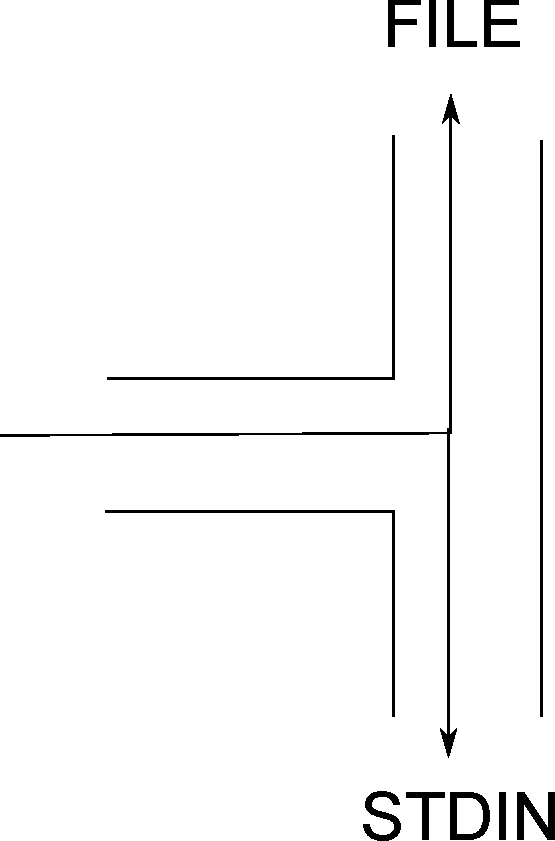
\includegraphics[width=.3\textwidth]{images/tee.pdf}
\end{frame}


\def\subsectitle{Bash comme vous ne l'avait jamais vu}
\subsection{\subsectitle}
\begin{frame}[containsverbatim]{\sectitle}
\begin{block}{\subsectitle}
\begin{verbatim}
while getopts a:bc:d option
do
case $option in
  a) echo "option a : $OPTARG";;
  b) echo "option b ";;
  c) echo "option c : $OPTARG";;  
  d) echo "la réponse d ";;  
esac
done
\end{verbatim}%$

\end{block}
\end{frame}

\begin{frame}{\sectitle}
\begin{block}{\subsectitle}
\begin{itemize}
\item Si un : suis l'option, alors on stocke un argument dans OPTARG
\item les options peuvent être regroupée -a p1 -bd
\item -dba p1
\item ...
\end{itemize}
\end{block}
\end{frame}

\def\subsectitle{Bash comme vous ne l'avait jamais vu}
\subsection{\subsectitle}
\begin{frame}[containsverbatim]{\sectitle}
\begin{block}{\subsectitle}
\begin{itemize}
\item \verb!bash -x! : mode debug
\item ou \verb!set -x! et \verb!set +x! dans un script
\end{itemize}


\end{block}


\begin{block}{Debug}
Permet d'afficher la ligne en cours d'exécution
\end{block}

\end{frame}


\def\subsectitle{Environnement bash}
\subsection{\subsectitle}
\begin{frame}[containsverbatim]{\sectitle}
\begin{block}{\subsectitle}
\begin{itemize}
\item .bash\_profile : personnaliser votre shell.
\item .bashrc : lorsque l'on lance sans login
\item \verb!/etc/profile!
\item \verb!/etc/bashrc!
\end{itemize}


\end{block}



\def\subsectitle{Personnaliser quoi}
\begin{block}{\subsectitle}
\begin{itemize}
\item  PS1, PS2...
\item alias de commande
\item script de démarrage
\item message d'accueil.
\end{itemize}
\end{block}
\end{frame}

\def\subsectitle{Un soucis??}
\subsection{\subsectitle}
\begin{frame}[containsverbatim]{\sectitle}
\begin{block}{\subsectitle}
\begin{center}
{\bf
R.T.F.M.

Read The Fucking Manual
}
\end{center}


\end{block}
\end{frame}

\begin{frame}[containsverbatim]{\sectitle}
\begin{block}{\subsectitle}
\begin{itemize}
\item \verb!man! commande
\item \verb!man man!
\end{itemize}
\end{block}
\end{frame}

\end{document}
